\documentclass[oribibl]{llncs}
 \usepackage{graphicx}
 \usepackage{subfigure}
\usepackage[utf8x]{inputenc}

\begin{document}

\title{Detection of chickenpox vesicles in digital images of skin lesions} %and discrimination from herpes zoster vesicles }
\author{Juli\'an Oyola, Virginia Arroyo, Ana Ruedin, Daniel Acevedo}
\institute{Departamento de Computaci\'on, Facultad de Ciencias Exactas y Naturales,\\ Universidad de Buenos Aires\\ Ciudad Universitaria, Pab. I. (C1428EGA), Ciudad de Buenos Aires\\
 \email{\{joyola, ana.ruedin, dacevedo\}@dc.uba.ar, virginia.arroyo@gmail.com}}
\maketitle
\begin{abstract} %75-150
Chickenpox is a viral disease characterized by itchy skin vesicles that can have severe complications in adults. A tool for automatic detection of these lesions in patients' photographs is highly desirable to help the physician in the diagnosis.
In this work we design a method for detection of chickenpox skin lesions in images. 
It is a combination of image processing techniques - color transform, equalization, edge detection, circular Hough transform-  and statistical tests. %  ***herpes zoster  and statistical tests
We obtain highly satisfactory results in the detection of chickenpox vesicles, the elimination of false detections using the Kullback Leibler divergence, and in preliminary tests for discrimination between chickenpox and herpes zoster. 
\end{abstract}
\keywords{skin lesions, chickenpox, detection, image processing}

\thispagestyle{empty}


\section{Introduction}
Chickenpox or varicella, caused by the varicella-zoster virus of the herpes group, is a very contagious infection that causes itchy outbreaks of skin vesicles.  The disease is spread by droplet or direct contact. The incubation period for chickenpox ranges from 11 to 21 days. Early symptoms consist of low-grade fever, headache, unrest and anorexia. 
On the following day, the characteristic rash begins to appear. The lesions evolve to form small papules, and then vesicles. 
Over the next several days, the vesicles rupture and then crust. The rash begins on the chest and back and spreads  to involve the face, scalp, and the extremities. 
New lesions of chickenpox arise in crops over a period of several days. 

This viral infection is most common amongst children, for whom it evolves as a mild disease: children recover uneventfully or with a few minor scars. However, teenagers and adults can also get chickenpox 
in which case it can be extremely severe. Complications from chickenpox include pneumonia, encephalitis, and skin infection; some of the mentioned complications can end in the patient's death.  Chickenpox can also lead 
to severe problems in pregnant women, causing birth defects of the newborn. Persons with weakened immune systems are also at risk for complications resulting from chickenpox. It is highly desirable to have a tool for 
early detection of chickenpox vesicles, specially in the case of adults.

After a chickenpox infection, varicella-zoster virus can become latent in the nerve cell bodies, 
 without causing any symptoms. Years or decades later, the virus can become active again, break out of nerve cell bodies and travel down nerve axons to cause viral infection of the skin in the region of the nerve, accompanied by headaches and sensitivity to light.
This disease is herpes zoster, also known as shingles or zona. Although the rash usually heals within two to four weeks, some patients experience residual nerve pain for months or years. 
It is also desirable to have a tool to distinguish chickenpox from herpes zoster. 


The object of this paper is to develop a method capable of detecting chickenpox vesicles, and analyze and extract their characteristics in order to discriminate them from other diseases, such as herpes-zoster. 
In the long run it is intended to become a part of a general tool designed 
to assist physicians in the task of diagnosing skin diseases.
To do this we apply a combination of image processing and pattern recognition techniques. These aim at increasing global contrast, detecting edges, detecting circles, and extracting color information. Global contrast is increased by histogram equalization, 
edges are detected with a Canny edge detector
, circles are detected by means of the circular Hough transform
, and color information is used twice: 
with the  Kullback Leibler divergence 
to eliminate false positives, and with statistical tests to discriminate chickenpox from herpes zoster. 

Databases with images of skin lesions -varicella vesicles,  
and other diseases- are difficult to find, and generally lacking. As a consequence, there is little or no research on such images. 
But many of the tools that we have integrated into our algorithm have been applied in the past. Histogram equalization has been used to improve contrast \cite{a_novel_approach_contrast}. 
A Canny edge detector was applied on facial recognition to detect 
facial expressions \cite{real_time_facial}. 
The circular Hough transform has been used to detect circular shapes in images, namely to find coconuts ~\cite{CH01}. 
Color information was used to detect other skin lesions, such as  
malignant melanoma \cite{LC01}.

This paper is organized as follows. In Sec.~2 we give some considerations on available images of skin lesions. Sec.~3 addresses the detection of chickenpox vesicles: edge detection, circular shape detection, elimination of duplicate detections, and elimination of false detections. In Sec.~4 we give concluding remarks.
\section{Some considerations on images of skin lesions}
The images we worked with for detection of varicella vesicles were downloaded from the University of Iowa website\footnote{http://www.lib.uiowa.edu/hardin/md/dermpictures.html}. %\cite{iowa}.
Great differences in the resolution, the scale and the lighting conditions were observed -- see Fig. \ref{fig_variacionesdeescala}. 
Moreover, there were variations
 in the colors of the patients' skin, as well as differences in the stages of the illness- skin rash in the early days, then vesicles, and finally crusts. All these differences contribute to the  difficulty  of detecting varicella from photographic images. 
Another added difficulty are hairs, moles and inscriptions present in the image.
In order to work with a more homogeneous set of images, we have discarded those having very small skin lesions, such as Fig. \ref{fig_variacionesdeescala}(a).
\begin{figure}
\centering
\subfigure[]
{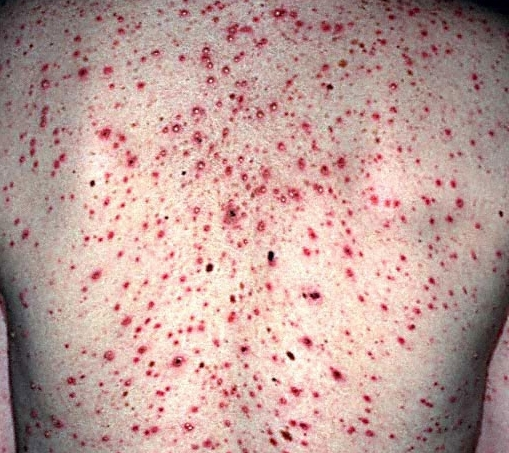
\includegraphics[width=0.22\textwidth]{Resources/chicken_pox_picture_01chi.jpg}}\hspace{2pt}
\subfigure[]
{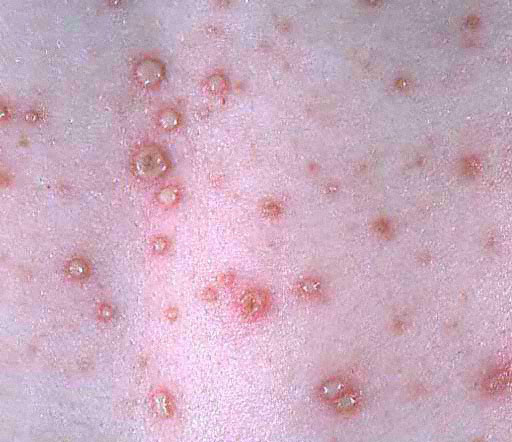
\includegraphics[width=0.23\textwidth]{Resources/chicken_pox_picture_13.jpg}}\hspace{3pt}% \\
\subfigure[]
{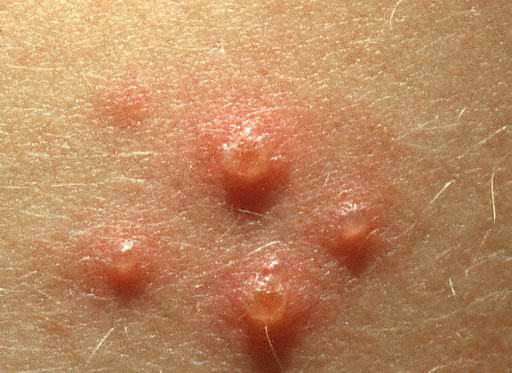
\includegraphics[width=0.27\textwidth]{Resources/chicken_pox_primary_lesions_03.jpg}}\hspace{3pt}%\hspace{15pt}
\subfigure[]
{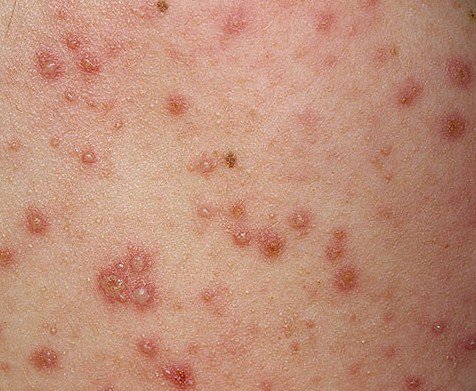
\includegraphics[width=0.24\textwidth]{Resources/rec_varicella_5.jpg}}
\caption{Varicella skin lesions of differently coloured skins, at different scales and different illumination conditions.\label{fig_variacionesdeescala}}
\end{figure}

\section{Detection of varicella vesicles}
\subsection{Luminance information for edge detection}
To increase global contrast in each image, histogram equalization was performed as a first step in the detection of skin vesicles.
Next the luminance component was extracted by converting the images to YCbCr and L*a*b* color spaces- both color representations separate luminance from chrominance.

To find the edges of an image we used a Canny edge detector \cite{JC01} on the luminance component. This detector is robust, and provides localized edges as well as connectivity of contours. 
It consists of 4 steps: Gaussian smoothing, gradient filtering, non-maximum suppression to obtain thin borders, and hysteresis thresholding.
Since chickenpox  vesicles are generally circular, extracted edges having circular shape are listed as candidates for vesicles.  
%
%
%
\subsection{Detection of circles}
The Circular Hough Transform was used to determine circular shapes in the
image of extracted edges. The classical version of this transform was first
introduced by Paul Hough in \cite{HO01} to detect lines in a binary image
and later it was popularized by Ballard \cite{BA81} for gray-scale images and arbitrary shapes. The rough idea behind the Hough transform is that every circle can be represented by a
center point and a radius (this is the parameter space in the Hough
transform). Then, for each point on an edge in the image plane (and for a
specific radius), circles are drawn and accumulated on a mask image. The following geometric property is used: %
\emph{given a circle with center $c$ and radius $r$, if along each point of the circumference we draw a circle --of radius  $r$-- centered upon that point, then all these  
circles will intersect at $c$}. 

The circles drawn -centered on the edge of the image - accumulate votes for the centre of a possible circle, if the shape of the edge is circular. %
We may detect circle-centers by searching for the most voted points in the accumulator mask \cite{SJ01}. This is done by trying with different circle radii (one accumulator 
mask for each radius). Given a circle with a determined radius, the number of points or pixels that lie on its border is known. Accordingly, the ideal number of votes that the center should have is also known. 
A circular shape is detected, when in the accumulator mask a  point has enough votes to exceed a given threshold-- a percentage (70 \% -- 90 \%) of the ideal score. 
In Fig. \ref{fig:deteccionRadios4043} we observe the edges of a vesicle, and detected circles with different radii. 
\begin{figure}[ht]
\centering
 \subfigure[]
{ 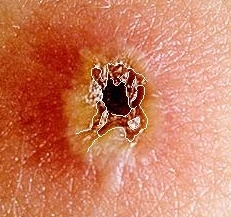
\includegraphics[scale=0.48]{Resources/resultado-varicella_18-bordesm.jpg} }\hspace{0.1pt}
 \subfigure[]
{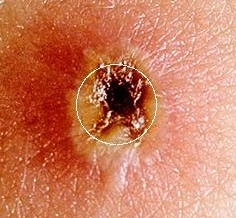
\includegraphics[scale=0.48]{Resources/resultado-varicella_18-radio40m.jpg}}\hspace{5pt}%\\
 \subfigure[]
{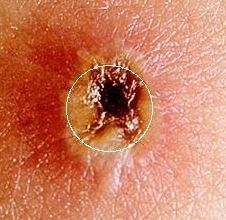
\includegraphics[scale=0.47]{Resources/resultado-varicella_18-radio43m.jpg}}
 \caption{In white: (a) edges of vesicle and circle detection with radii (b) $r = 40$ and (c) $r = 43$.  \label{fig:deteccionRadios4043}}
\end{figure}
In Fig. \ref{fig:umbralPorcentajeHough} we observe the edges of the image, where some edges are circular and some (marked in red) are only approximately circular. Circles detected with thresholds  70\% and 90\% are also shown. 
Notice that with a threshold of 70\%, some spurious circles - false positives- are detected, as well as the approximately circular vesicles; these disappear with the  90\% threshold.
\begin{figure}
\centering
\label{fig:bordesDetectados}
\subfigure[]{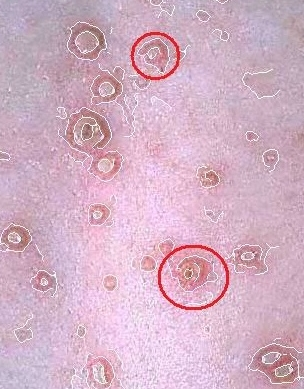
\includegraphics[width=0.32\textwidth]{Resources/resultado-chicken_pox_picture_13-marcadom.jpg}}
\subfigure[]{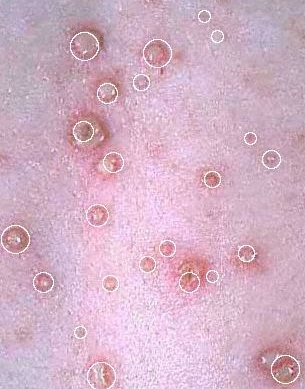
\includegraphics[width=0.32\textwidth]{Resources/resultado-chicken_pox_picture_13-int689101114-conc2-70m.jpg}}
\subfigure[]{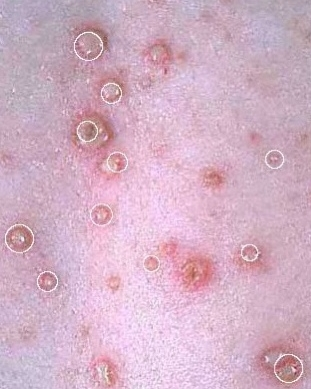
\includegraphics[width=0.327\textwidth]{Resources/resultado-chicken_pox_picture_13-int689101114-conc2-90m.jpg}}
\caption{(a) Vesicles and detected edges in white. Some edges having a very approximate circular shape are marked in red. (b) Circles detected with a threshold of 70\%, in white.  (c) Circles detected with a threshold of 90\%, in white.} 
\label{fig:umbralPorcentajeHough}
\end{figure}
\subsection{Dealing with duplicate detected circles}
When detecting circles it may happen that duplicate detections occur, or that the algorithm finds a profusion of circles near the same spot. We have chosen 2 different criterions to decide that 2 circles are in this situation:
\begin{itemize}
\item[{\it i})] We consider a case of duplicate detections when circle $C(c^{(a)}, r_a)$ (having center $c^{(a)}$ and radius $r_a$) and circle $C(c^{(b)}, r_b)$, satisfy \mbox{ $ \left\| c^{(a)} - c^{(b)}  \right\| \! < \max\{r_a,r_b\}$}, 
in which case the center of the smaller circle is inside the larger one. \\
\item[{\it ii})] We consider a case of duplicate detections when circles $C(c^{(a)}, r_a)$, $C(c^{(b)}, r_b)$, satisfy   $\left\| c^{(a)} - c^{(b)} \right\| < r_a+r_b$, in which case both circles intersect.
\end{itemize}
%
In the presence of duplicate detections we eliminate the circle having less votes in the acumulator mask. In Fig. \ref{fig:deteccionDuplicadosK1K2} we show the result of eliminating duplicate circles with each criterion, 
the second criterion being the one giving better results.
%
%
 \begin{figure}
 \centering
\subfigure[]
{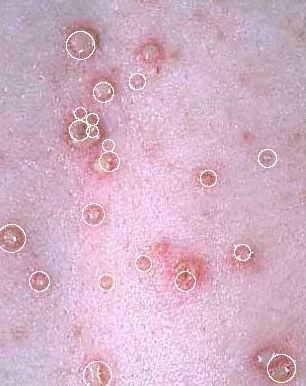
\includegraphics[scale=0.36]{./Resources/resultado-chicken_pox_picture_13-int689101114am.jpg}}\hspace{15pt}
\subfigure[]
{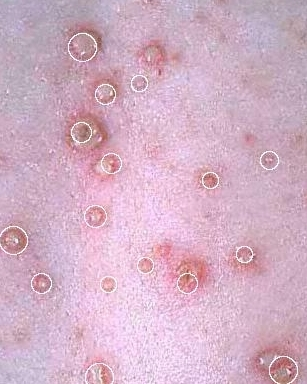
\includegraphics[scale=0.36]{./Resources/resultado-chicken_pox_picture_13-int689101114-conc2m.jpg}}
\caption{(a) Result of eliminating duplicate circles with criterion \textit{i}). (b) Result of eliminating duplicate circles with criterion \textit{ii}) --see text.
 \label{fig:deteccionDuplicadosK1K2}}
\end{figure}
\subsection{Chrominance information to eliminate false positives}
 As mentioned earlier, the original RGB images were transformed to L*a*b* color space. The CIE L*a*b* was specified by the ``Commission internationale de l'éclairage'',  
its aim was that uniform changes of components in the L*a*b* color space would correspond to uniform changes in perceived color.
To eliminate false vesicle detections, we worked on component a* of this color representation. 
The pixels inside each detected vesicle were extracted, and their a* chromatic component was analyzed. 
First we calculated the empirical histogram of all the pixels in the true varicella vesicles.
The Kullback Leibler distance between this all-varicella-histogram and the empirical histograms of each detected circle, whether it were a false positive(skin) or true positive (varicella). 
In Table \ref{tabla} we list the KLD between histograms of 10 false detection -and 10 true detections - versus the histogram of all varicella pixels. Notice that false detections all have much higher KLD values, which helps to 
get rid of these false positives.

\begin{table}% [ht]
\centering
\begin{tabular}{@{\quad}c|@{\quad}l@{\quad}l@{\quad}l@{\quad}l@{\quad}l@{\quad}l@{\quad}l@{\quad}l@{\quad}l@{\quad}l}
  Skin &  24.26 &   25.30   & 23.94   & 23.63  & 27.54   & 28.98      & 38.66       & 25.71    & 18.89  & 22.52    \\ \hline
Varicella  & 0.334 &  0.515  &  1.131   &  0.679   &  2.771   &  2.005    &   2.168     &  0.684    & 1.486   &  1.833
\end{tabular}
\vspace{0.1in}
\caption{\small{Row 1: KLD between empirical histogram of pixels (component a*) inside 10 spurious detected circles versus the histogram of all varicella pixels (component a*).
Row 2: KLD between empirical histogram of pixels (component a*) inside 10 truly detected varicella vesicles versus the histogram of all varicella pixels (component a*).} \label{tabla} }
\end{table}

\section{Discriminating between chickenpox and herpes zoster vesicles}

We have made preliminary tests in order to discriminate chickenpox vesicles from herpes zoster vesicles. These we carried out on 4 images - see 
Fig. \ref{fig:varicelayherpeszoster}\footnote{The original images (chickenpox\_primary\_lesions\_03, varicella\_34, herpes\_zoster\_114, herpes\_zoster\_8) are larger. A detail containing all detected vesicles is shown.}.

\begin{figure}[h]
\centering
\subfigure[]
{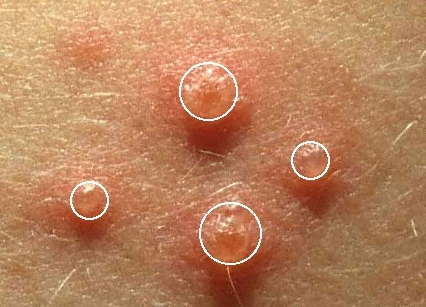
\includegraphics[width=0.32\textwidth]{Resources/chicken_pox_primary_lesions_03_concirculos_crop.jpg}}\hspace{4pt}
\subfigure[]
{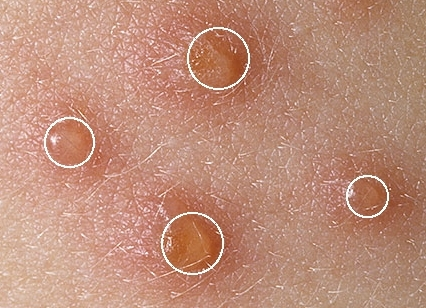
\includegraphics[width=0.32\textwidth]{Resources/varicella_34_concirculos_crop.jpg}}\hspace{4pt} \\
\subfigure[]
{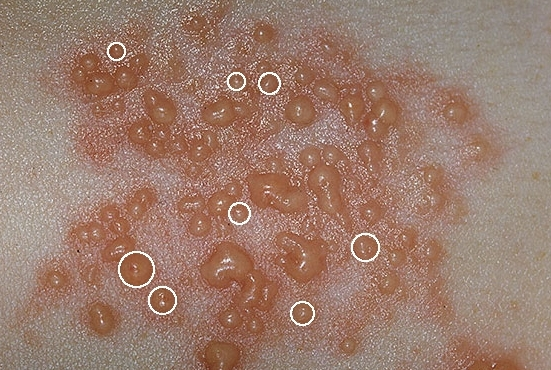
\includegraphics[width=0.32\textwidth]{Resources/herpes_zoster_114_concirculos_crop.jpg}}\hspace{4pt}\hspace{0.5pt}
\subfigure[]
{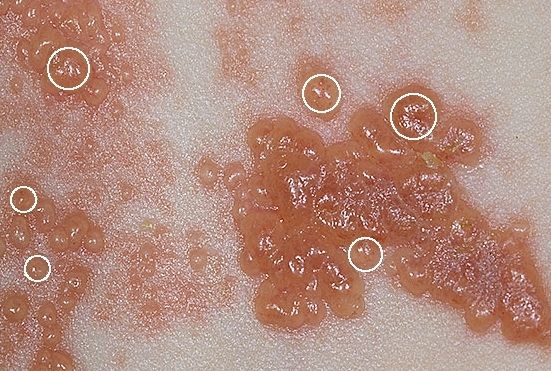
\includegraphics[width=0.32\textwidth]{Resources/herpes_zoster_8_concirculos_crop.jpg}}
\caption{Skin lesions and detected vesicles. (a) - (b) Examples of chickenpox lesions. (c) - (d) Examples of herpes zoster lesions.\label{fig:varicelayherpeszoster}}
\end{figure}


Different tests were performed on the 3 components of L*a*b* color system, assuming normal distributed values and equal variances in the data. We found statistical evidence of differences between the means of the 2 classes (chickenpox and herpes zoster) on component a*. This component indicates the position of the pixel's color between green and red/magenta (a* negative values indicate green, while positive values indicate magenta). 
In Fig. \ref{fig:histogramas} are given the histograms of component a* in the vesicles of each image of Fig. \ref{fig:varicelayherpeszoster}. 
Notice that the sample means are much smaller for herpes zoster lesions than for chickenpox lesions.

\begin{figure}
\centering 
\subfigure[$\bar{x}=29.2, N=7284$]{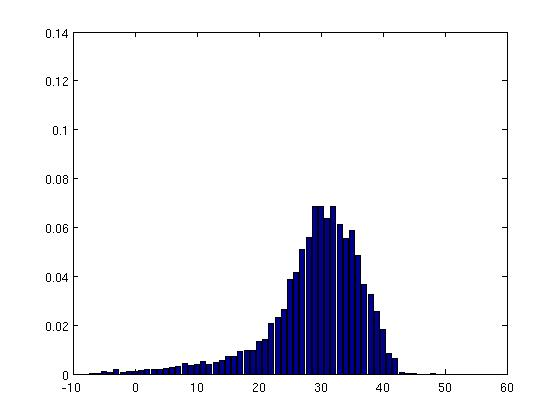
\includegraphics[width=0.32\textwidth]{Resources/chickenpox03_C2_hist.jpg}}%\hspace{2pt}
\subfigure[$\bar{x}=26.6, N=8684$]{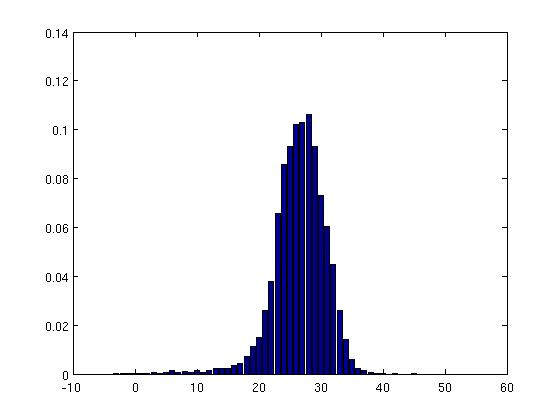
\includegraphics[width=0.32\textwidth]{Resources/varicella_34_C2_hist.jpg}} 
\subfigure[$\bar{x}=20.0, N=3348$]{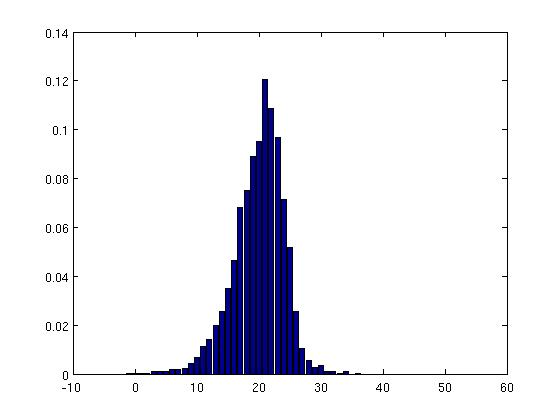
\includegraphics[width=0.32\textwidth]{Resources/HerpesZoster114_C2_hist.jpg}}%\hspace{2pt}%\hspace{15pt}
\subfigure[$\bar{x}=23.1, N=5450$]{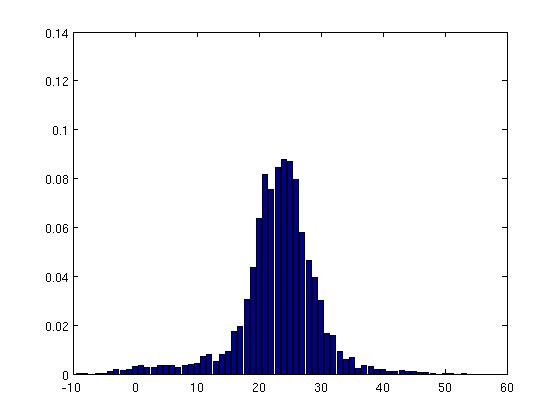
\includegraphics[width=0.32\textwidth]{Resources/HerpesZoster8_C2_hist.jpg}}
\caption{Histograms of component a* of pixels inside vesicles, $\bar{x}$ is the sample mean, $N$ is the number of samples; (a) - (b): chickenpox lesions; (c) - (d): herpes zoster lesions.\label{fig:histogramas}}
\end{figure}



An ANOVA (Analysis of variance) test was carried out to compare the mean values of pixels (component a*) belonging to the 2 classes.  There were $N=15968$ samples in the chickenpox class, and $N=8798$ samples in the herpes zoster class. 
With probability 1 ($p=0$) the null hypothesis --that the means of the 2 classes are equal-- was rejected. The estimated value for the difference between the means was $\mu_{\scriptsize\textrm{(chickenpox)}}- \mu_{\scriptsize\textrm{(herpeszoster)}} =5.8608$, with a 100\% confidence interval of  [5.7044,  6.0171]. The test 
indicates that the error between classes was much greater than the intraclass error.   

Next four vectors were built gathering information from inside the vesicles of each mentioned image (component a*). An ANOVA was performed on these four vectors, and multiple comparisons were done between the vectors. 
We list the estimated value for the difference between the means, and give the  100\% confidence intervals. Recall that (a) and (b) belong to chickenpox class, (c) and (d) to herpes zoster class.\\
Interclass comparisons:\\
$\mu_{(a)}- \mu_{(c)} =  9.1967      \in [   8.8831    , \      9.5104    ]$;  
$\mu_{(a)}- \mu_{(d)} =   6.1135      \in [  5.8445     , \      6.3826    ]$.  
$\mu_{(b)}- \mu_{(c)} =  6.5746      \in  [   6.2689    , \      6.8802     ]$;  
$\mu_{(b)}- \mu_{(d)} =   3.4913       \in [ 3.2317      , \     3.7509    ]$.  
Intraclass comparisons:\\
$\mu_{(a)}- \mu_{(b)} =  2.6222       \in [   2.3835 , \       2.8609    ]$;  
$\mu_{(c)}- \mu_{(d)} =   -3.0832         \in [ -3.4131, \     -2.7533 ]$.  
 

From these results we conclude that there is sufficient statistical evidence to
reject the (null) hypothesis that the difference between the means of 2 images
belonging to different classes is 0 (i.e., the means of images belonging to
different classes are significantly different).
However, although the difference of means was smaller for intraclass comparisons than for interclass comparisons, there is too much variability in the data to be able 
to accept the other (null) hypothesis that images belonging to the same class have equal means. The last 2 confidence intervals should have contained 0 to be able to accept this hypothesis.

\section{Conclusions}
A tool for detection of chickenpox vesicles was designed, giving satisfactory results when applied over a group of pictures belonging to patients that suffer from this illness. 
Most vesicles were successfully detected by applying different image processing and pattern recognition techniques, and the method has proven to be robust under different illumination scenarios. 
Both lumninance and chrominance information were used to obtain result. Once vesicles were detected, preliminary statistical tests for discrimination between herpez zoster and chickenpox classes achieved promising results, although intraclass variance was high.


\bibliographystyle{splncs}

\begin{thebibliography}{20}

\bibitem{a_novel_approach_contrast}
H. Yeganeh, A. Ziaei, A. Rezaie.
``A novel approach for contrast enhancement based on Histogram Equalization'',
IEEE Int. Conf. Computer and Communication Eng., pp. 256-260, 2008. 

\bibitem{real_time_facial}
Peng Zhao-yi, Zhu Yan-hui, Zhou Yu
``Real-time Facial Expression Recognition Based on Adaptive Canny Operator Edge Detection'',
IEEE Int. Conf. Multimedia and Information Technology, pp. 154-157, 2010. 

\bibitem{CH01} M. Rizon, H. Yazid, P. Saad, A. Md Shakaff, A. Saad, M. Sugisaka, S. Yaacob, M. Mamat, M.Karthigayan.
``Object Detection using Circular Hough Transform'',
American Journal of Applied Sciences 2 (12), pp. 1606-1609, 2005.

 \bibitem{LC01} L. Coll, D. Chinchilla, C. Coll, F. Stengel, H. Cabo.
 ``Análisis digital de imágenes en lesiones pigmentadas de la piel. Diagnóstico precoz del melanoma'', Dermatología Argentina, vol. 14, No. 3, 2008.
 
\bibitem{JC01} J.F. Canny.
``A Computational Approach to Edge Detection'', 
\emph{IEEE PAMI}, 8(6), 1986, pp. 679-698.

\bibitem{HO01} Hough, P. V. 
``Machine analysis of bubble chamber pictures''. Int. Conf. on High Energy Accelerators and Instrumentation'', (L. Kowarski, ed.) pp 554--556, 1959.


\bibitem{BA81} D.H. Ballard,``Generalizing the Hough Transform to Detect
Arbitrary Shapes'', Pattern Recognition, Vol.13, No.2, pp. 111-122, 1981.

\bibitem{SJ01} Simon Pedersen.
``Circular Hough Transform'',
Aalborg University, Vision, Graphics, and Interactive Systems, November 2007.

\end{thebibliography}


\end{document}


